\section{Motivation}

\begin{figure*}[h]
    \centering
      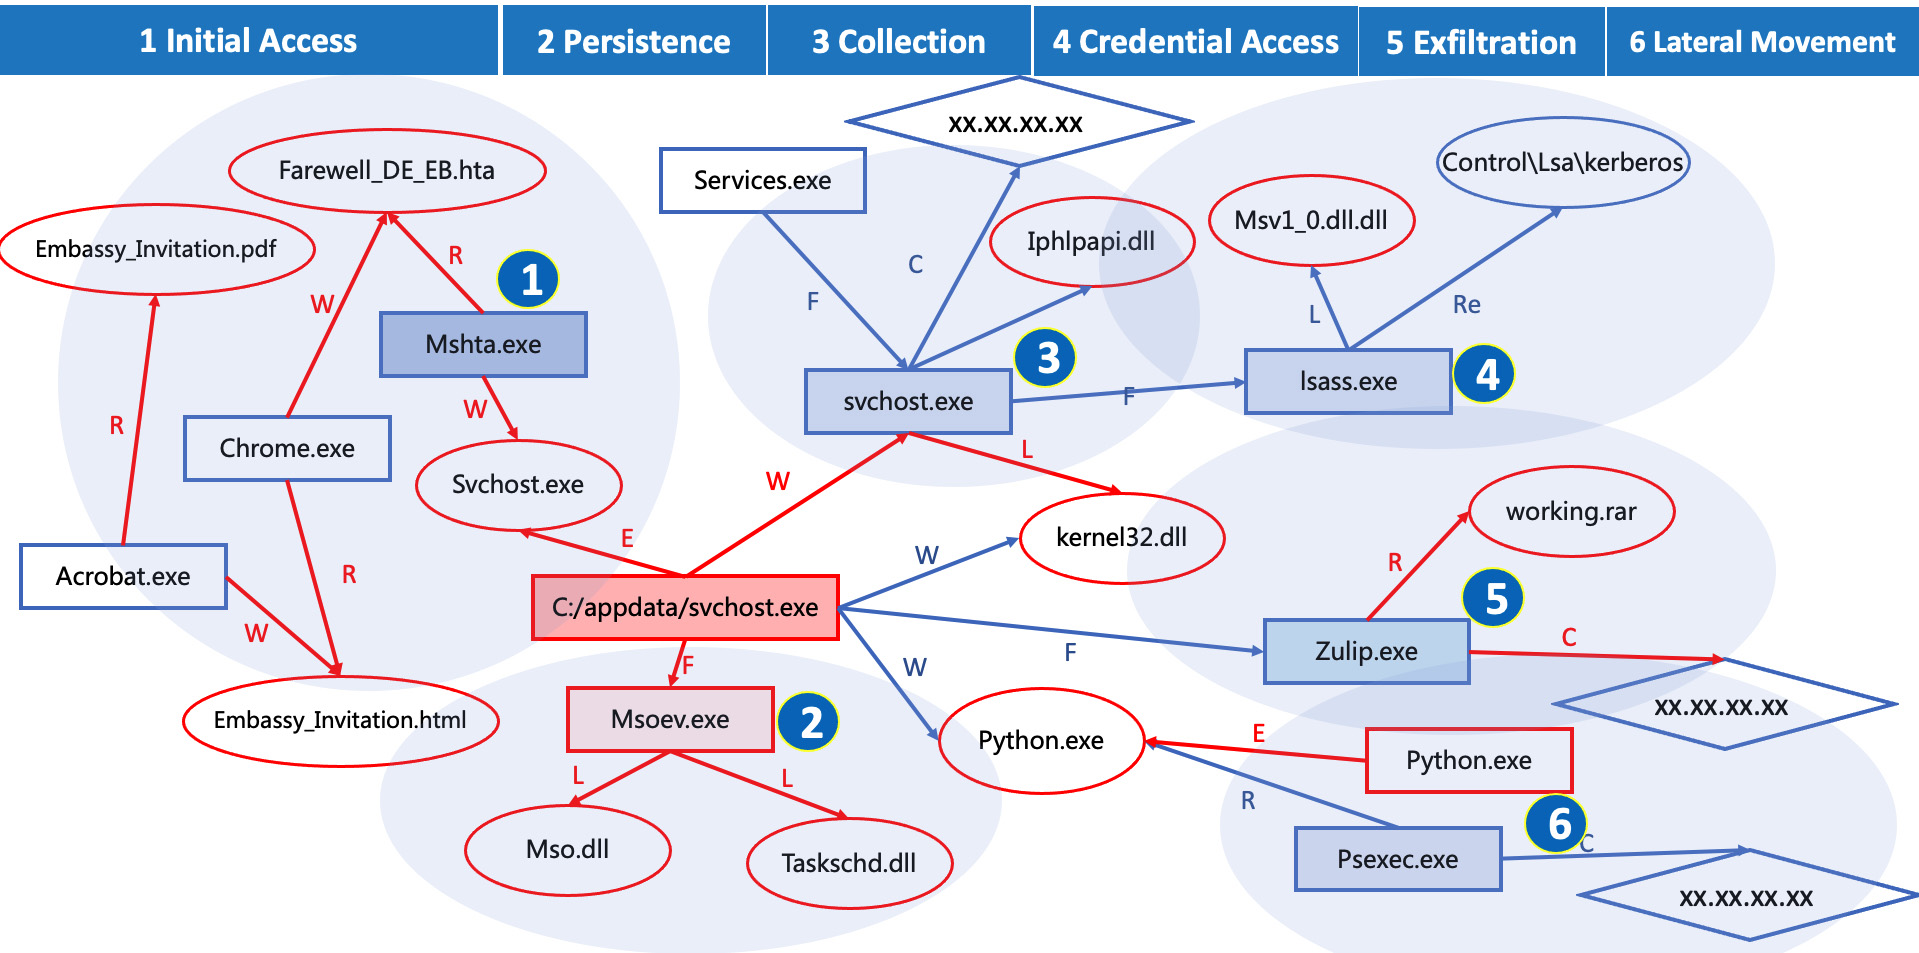
\includegraphics[width=1\textwidth]{figs/example.jpg}
    \caption{A provenance summary graph from APT29 that describes attack activity in the motivating example, as automatically generated by ProCon. Rectangles, ovals, and diamonds represent processes, files, and sockets, respectively. R=Read, W=Write, O=Open, S=Send, Re=Register, F=Fork, and E=Execute. We have segmented the attack progression into six distinct steps, with each step delineated by a light blue shaded backdrop. Central to each phase is a pivotal process, symbolized by a solid entity. Elements pertinent to the attack are highlighted in red, while those signifying regular events and nodes are depicted in blue.}
    \label{fig-example} 
    \end{figure*}

We use a real-world APT attack to illustrate the limitations of current detection methods and the intuition behind our approach.
\subsection{Motivating Example}
The "German Embassy Invitation Lure" is a real-world APT attack attributed to APT29, a notorious Russian attack group. By blending the original attack strategies with the stealthy tactics often deployed by APT29, we simulated a new APT attack scenario. This assault initiates with a deceptively authentic phishing email targeting diplomats, seemingly sent from the German embassy
The main attack vector was a seemingly harmless PDF attachment in the email. However, upon downloading and opening this document, victims inadvertently activated concealed malicious code.
In the aftermath of this initial breach, ostensibly benign programs, such as Mshta.exe, went into overdrive, downloading and executing a program disguised as "svchost.exe" within the directory c:/appdata/. This camouflaged svchost.exe then utilized a DLL Side-Loading technique involving "Msoev.exe" to load a malicious DLL masked as "Mso.dll." This DLL harbored functionalities to establish persistence in the compromised system.

The plot thickened as the malicious version of svchost.exe then proceeded to inject another harmful DLL, masked as "kernel32.exe," into the legitimate svchost.exe of the system. This malevolent DLL had the capabilities to scan the network, identifying potential new targets for infiltration.
Exploiting a vulnerability, the attackers downgraded the Kerberos protocol to the more vulnerable MSV protocol. This move allowed them to pilfer credentials from the domain, setting the stage for lateral movement within the network. Simultaneously, "Zulip.exe" was deployed by the attackers, aiding in data exfiltration.
In the attack's final phase, the assailants wielded "psexec.exe" in conjunction with the previously stolen credentials. This combination allowed them to remotely execute a malicious program camouflaged as "python.exe," facilitating lateral movement to a fresh host.

Figure~\ref{fig-example} showcases a simplified provenance graph constructed from audit records of the Embassy Lure. The nodes in the graph signify system entities. Rectangles, ovals, and diamonds represent processes, files, and sockets, respectively. Gray edges reflect system calls oriented in the direction of information flows. For clarity, unique nodes are used in the graph to represent distinct instances, such as individual processes or different network connections. This provenance graph serves as a potent representation tool, allowing analysts to navigate extensive audit records seamlessly. It aids security experts in backward and forward information flow tracking, enabling the identification of root causes behind security breaches and understanding their ramifications.


\subsection{Challenge to Existing Solutions}
Limitations of Provenance-Based Threat Detection in the Embassy Lure Attack:

\begin{itemize}
    \item \textit{Statistics-based Detection}: While provenance-based approaches are adept at identifying potential threats within graphs, they frequently misinterpret benign but rare activities as malicious. For instance, in scenarios akin to the Embassy Lure attack, svchost.exe can host multiple services. Hosting the Connected Devices Platform (CDP) service, which manages device connections, is a rarity. Consequently, statistics-based approaches would likely flag it as malicious. Moreover, the outcomes from these statistical methods lack interpretability.
    \item \textit{Misuse-based Detection}: Misuse-based detectors search for cyber threats by matching audit records against a knowledge base of security policies that describe attack semantics. While such detection can maintain a low false-positive rate, the creation of these security policies is time-intensive and necessitates domain expertise. Pertaining to our example, a single TTP can correspond to numerous specific attack techniques. For instance, while "initial access" encompasses various implementation methods, our case employed Mshta.exe. Experts are tasked with covering all attack behaviors for a given TTP, a process which is not only labor-intensive but also falls short when encountering unknown or evolving attacks.Furthermore, factors like experts' subjective interpretations of attacks, varying proficiency levels, or even simple human errors can lead to significant disparities in the quality of the formulated policies.
    \item \textit{Anomaly-based Detection}: Anomaly-based detection techniques, while skilled at detecting deviations, often grapple with providing an in-depth understanding of the underlying attack mechanisms. In scenarios akin to the Embassy Lure attack, the deluge of records can easily overwhelm security analysts, making the root cause identification a daunting task. Solutions like Unicorn might trigger alerts across an entire graph, yet lack the precision to indicate which specific entities or patterns. These attacks may craft patterns that skillfully mirror benign activities, rendering them virtually imperceptible. The scarcity of anomalous data in comparison to the vast majority of benign logs (with malicious entries sometimes representing less than 1\% of the total) amplifies the complexity. Meanwhile, due to the limited representation of these stealthy threats in the logs, training a robust and reliable model becomes a formidable challenge. Moreover, savvy attackers can potentially exploit these vulnerabilities, further evading detection.In our example, the attack behaviors are highly stealthy. Anomaly detection tends to identify more macro-level behaviors, often missing such stealth activities.
\end{itemize}
In essence, each of these methods struggles to swiftly and accurately identify attacks. Furthermore, they often lack the granularity needed to elucidate and pinpoint specific attack behaviors, making the detection and subsequent response phases more challenging.



\subsection{Intuition of Our Approach}
Upon meticulously analyzing numerous APT attack reports, we discerned that attackers frequently employ a variety of subterfuge techniques to cloak their malicious undertakings. Among these techniques are masquerading as a legitimate process, spoofing the Parent Process ID, hollowing out a genuine process to inject malicious code, employing process injection, side-loading DLLs, and disguising by mimicking legitimate functionalities.

Interestingly, the stealthiness of these disguises tends to increase as attackers transition from straightforward masquerading techniques, like mimicking legitimate processes, to more sophisticated methods like functional masquerade.

A pivotal observation was that, irrespective of the masquerading method, there exist inherent constraints tied to genuine program behavior—execution paths, parent-child process relationships, permissions, and more. These constraints stand inviolable. In our attack scenario, we noticed stark deviations from these norms. For example, while a legitimate svchost.exe process typically has services.exe as its parent, the malicious variant in our case was spawned by Mshta.exe. Moreover, its execution path was not what one would anticipate for an authentic svchost.exe.

For more stealth attacks, like process injection, the maliciously injected kernel32.dll disrupts the expected load chain and violates the associated temporal constraints. This emphasizes that even as attackers innovate, their strategies are likely to infringe upon some established constraints, making the establishment of profiles and constraints for regular processes crucial in bolstering APT attack detection.

% \cite{inam2022sok}
% \cite{wang2022threatrace}
% \cite{zeng2021watson}
% \cite{zengy2022shadewatcher}
% \cite{alsaheel2021atlas}
% \cite{wang2020you}
